%% The first command in your LaTeX source must be the \documentclass command.
%%
%% Options:
%% twocolumn : Two column layout.
%% hf: enable header and footer.
\documentclass[
% twocolumn,
% hf,
]{ceurart}

%%
%% One can fix some overfulls
\sloppy

%%
%% Minted listings support 
%% Need pygment <http://pygments.org/> <http://pypi.python.org/pypi/Pygments>
\usepackage{caption}
% \captionsetup{format=plain}
\captionsetup[table]{format=plain,labelformat=simple,labelsep=period}

\usepackage{listings}
% \usepackage{multirow}

%%
%% end of the preamble, start of the body of the document source.
\begin{document}

%%
%% Rights management information.
%% CC-BY is default license.
\copyrightyear{2025}
\copyrightclause{Copyright for this paper by its authors. Use permitted under Creative Commons License Attribution 4.0 International (CC BY 4.0).}

%%
%% This command is for the conference information
\conference{ISWC 2024 Special Session on Harmonising Generative AI and Semantic Web Technologies, November 13, 2024, Baltimore, Maryland}

%%
%% The "title" command
\title{LLM-based SPARQL Query Generation from Natural Language over Federated Knowledge Graphs}

%%
%% The "author" command and its associated commands are used to define
%% the authors and their affiliations.
\author[1]{Vincent Emonet}[%
orcid=0000-0002-1501-1082,
email=vincent.emonet@sib.swiss,
% url=https://vemonet.github.io,
]
\cormark[1]
%\fnmark[1]
\address[1]{SIB Swiss Institute of Bioinformatics, Switzerland}

\author[1]{Jerven Bolleman}[%
orcid=0000-0002-7449-1266,
email=Jerven.Bolleman@sib.swiss,
%url=https://kmitd.github.io/ilaria/,
]

\author[1]{Severine Duvaud}[%
orcid=0000-0001-7892-9678,
email=severine.duvaud@sib.swiss,
]

\author[1]{Tarcisio {Mendes de Farias}}[%
orcid=0000-0002-3175-5372,
email=tarcisio.mendes@sib.swiss,
]

\author[1]{Ana Claudia Sima}[%
orcid=0000-0003-3213-4495,
email=ana-claudia.sima@sib.swiss,
]

%% Footnotes
\cortext[1]{Corresponding author.}
%\fntext[1]{These authors contributed equally.}

%% 
%% The abstract is a short summary of the work to be presented in the
%% article.
\begin{abstract}
We introduce a Retrieval-Augmented Generation (RAG) system for translating user questions into accurate federated SPARQL queries over bioinformatics knowledge graphs (KGs) leveraging Large Language Models (LLMs). To enhance accuracy and reduce hallucinations in query generation, our system utilises metadata from the KGs, including query examples and schema information, and incorporates a validation step to correct generated queries. The system is available online at \href{https://chat.expasy.org}{chat.expasy.org}. 
\end{abstract}

% We introduce a Retrieval-Augmented Generation (RAG) system for translating user questions into accurate federated SPARQL queries over bioinformatics knowledge graphs (KGs) leveraging Large Language Models (LLMs). We use the KG schemas to mitigate hallucinations in the generated queries, and we assist users in understanding and validating the generated queries by pointing out similar reference queries available, as well as providing human-readable explanations. The system is available online at \href{https://chat.expasy.org}{chat.expasy.org}. 

%%
%% Keywords. The author(s) should pick words that accurately describe
%% the work being presented. Separate the keywords with commas.
\begin{keywords}
  Knowledge Graph Question Answering \sep
  Federated SPARQL query \sep 
  Large Language Models \sep 
  Retrieval-Augmented Generation \sep
  SPARQL query generation
\end{keywords}

%%
%% This command processes the author and affiliation and title
%% information and builds the first part of the formatted document.
\maketitle

\section{Introduction}

In bioinformatics, the ability to query complex knowledge graphs (KGs) is critical for extracting meaningful insights. However, manually crafting SPARQL queries, especially federated queries spanning across multiple connected KGs, can be a time-consuming and challenging task, even for experts. This has led to a growing demand for Knowledge Graph Question Answering (KGQA) systems that can translate natural language queries into SPARQL, bridging the gap between users' questions and the structured data available. 

Large Language Models (LLMs) present an exciting opportunity to address this challenge, offering the potential to automatically generate accurate SPARQL queries from natural language inputs. However, while LLMs have demonstrated impressive capabilities in this area \cite{sima2023potential}\cite{meyer2024assessingsparqlcapabilitieslarge}, current systems struggle to handle large-scale, evolving KGs, such as those in the SIB Swiss Institute of Bioinformatics catalog \cite{sib2024sib}.

In this work, we present a solution designed to assist users of SIB’s bioinformatics KGs\cite{sima2019enabling}, such as UniProt \cite{uniprot2023uniprot}, Bgee \cite{bastian2021bgee} or OMA \cite{altenhoff2024oma}, to explore and query the data available. Our approach leverages LLMs and endpoints metadata to generate SPARQL queries while addressing the challenge of dynamically integrating evolving datasets, without requiring constant retraining. By offering a scalable system\footnote{\href{https://github.com/sib-swiss/sparql-llm}{github.com/sib-swiss/sparql-llm}} that adapts to the complex and changing landscape of bioinformatics knowledge, we aim to significantly reduce the time and expertise needed to query across federated KGs.

% The need for KGQA, the gap in systems that translate questions to federated queries, the opportunity with LLMs, the SIB catalog of federated real-world KGs and the large collection of example queries. The difficulty and time it takes to write complex queries across multiple knowledge graphs.

% The capabilities of LLMs to write SPARQL queries\cite{meyer2024assessingsparqlcapabilitieslarge}

% Our particular problematic: really large KGs, providing a system that enables to easily integrate new infos from those KGs that are evolving overtime without the need for retraining everything


% 1 motivating example to be used throughout paper (a concrete question and corresponding query), e.g. "Retrieve drugs that target human enzymes involved in sterol metabolism".

%%\section{Related works}
%%
%%% There have been works about SPARQL query generation. But most current paper are working on knowledge base using with small controlled ontologies. None for federated queries over multiple real-world knowledge bases where each endpoint has a complex schema involving multiple ontologies.
%%
%%A lot of existing works looked into training a model specifically for the query generation task, but modern LLMs are already pretrained well enough on publicly available SPARQL queries to usually generate syntactically correct SPARQL queries\cite{meyer2024assessingsparqlcapabilitieslarge}, the problem lies more on writing queries using the right semantics (classes and predicates), and identifiers.
%%
%%Retrieval-Augmented Generation gives good opportunities to be able to easily change the underlying LLM model and take advantages of latest advances, without the need to train new models everytime a KG has changed. And enable our syste to integrate new KG quickly on the fly.
%%
%%Some looked into training a custom model based on the KG structure\cite{SGPT}\cite{bustamante2024sparql}, it is an interesting approach that would lead to using smaller, less expensive models to run at inference. But when working with large KGs that are evolving over time, the training process could become expensive and time-consuming. Moreover we would like to leverage LLM explaining capabilities to give users better explanation of the generated queries.
%%
%%There has been work to fine-tune LLMs using sets of examples queries for life science knowledge graph\cite{rangel2024sparql}, this improved the quality of generated queries, which could be an interesting approach to take in order to be able to use smaller cheaper model for query generation.
%%
%%
%%Some research\cite{kovriguina2023sparqlgen} showed that providing context about a KG in the prompt such as a RDF subgraph related to the question can enable to achieve results close to pretrained models in some cases.
%%
%%
%%% \href{https://arxiv.org/html/2409.05925v1}{Assessing SPARQL capabilities of Large Language Models}: LLMs have no problem with query syntax. Find that existing KGQA benchmarks have ambiguity that hinder a proper automatic evaluation. Provides a Framework and task collection for automated benchmarking of Large Language Models (LLMs) on Knowledge Graph (KG) related tasks.
%%
%%\href{https://arxiv.org/pdf/2311.09841}{Leveraging LLMs in Scholarly Knowledge Graph Question Answering}: 
%%
%%
%%% Approaches based on schema approaches have been considered for a long time to generate queries:
%%% https://dl.acm.org/doi/pdf/10.1145/2187836.2187923
%%% GMark: Schema-driven generation of graphs and queries
%%
%%Regarding Retrieval-Augmented Generation here is what has been done, 
%%
%%Taffa \& Usbeck \cite{taffa2023leveraging} identifies the top-n similar training questions related to a given test question via a BERT-based sentence encoder and retrieves their corresponding SPARQL. Using the top-n similar question-SPARQL pairs as an example and the test question creates a prompt. Then pass the prompt to the LLM and generate a SPARQL. Finally, runs the SPARQL against the underlying KG - ORKG (OpenResearch KG) endpoint and returns an answer. The system achieves an F1 score of 99.0\%, on the SciQA\cite{sciqa2023} dataset- one of the Scholarly-QALD-23 challenge benchmarks (https://ceur-ws.org/Vol-3592/). This paper shows that using example queries provided as context to the LLM is an efficient method to generate accurate SPARQL queries.
%%
%%Rajpal \& Usbeck\cite{rajpal2024bertologynavigator} looked into entity linking using text embeddings for the user question and cosine similarity to find the most similar class in the KG. They show that in real world settings entity linking using embeddings to pick the most relevant class had limitations, but they still got 56\% of the matches correct. But there were only picking the most similar result, and not looking into the \textit{n} most similar results.
%%
%%Avila et al.\cite{avila2024experiments} implemented RAG for SPARQL query generation by indexing all classes and instances of the KG and used full-text search to find documents relevant to the user question. And build a small subgraph that is passed to the LLM as context. They then generated 5 queries to answer the question based on context, and try to execute each of them. Their benchmark was composed of a few relatively simple questions but achieved good results.
%%
%%
%%% Some approaches\cite{bustamante2024sparql} to tackle the DBLP-QuAD\cite{Dblp-quad} dataset have shown that separating the task of entity linking and query generation leads to good results. Performing entity linking in the huge knowledge graphs containing billions of biomedical entities is a really complex task by itself, requiring to build large entity search indexes. In this paper we are focusing on SPARQL query generation, but entity linking will be necessary for future improvement of SPARQL generation
%%
%%% There is a benchmark framework proposed recently bu meyer2024 https://github.com/AKSW/LLM-KG-Bench
%%
%%Benchmark datasets:
%%
%%TODO: Checkout existing benchmark datasets, and benchmark frameworks, and explain how the test suite we propose makes sense regarding those existing systems.
%%
%%- DBLP-QuAD\cite{Dblp-quad}, while it is large (10.000 question/answer pairs), the question are relatively simple, maximum to 2 hops. Most of the challenge lies in entity extraction and linking, which is not our goal at the moment. Meanwhile the average number of triple pattern in our example is XX
%%
%%- M. Dubey, D. Banerjee, A. Abdelkawi, and J. Lehmann, ‘‘LC-QuAD 2.0: A large dataset for complex question answering over Wikidata and DBpedia,’’ in Proc. Int. Semantic Web Conf. Auckland, New Zealand: Springer, 2019, pp. 69–78.
%%
%%- E. Kacupaj, H. Zafar, J. Lehmann, and M. Maleshkova, ‘‘VQuAnDa: Verbalization question answering dataset,’’ in Proc. Eur. Semantic Web Conf. Heraklion, Greece: Springer, 2020, pp. 531–547
%%
%%- QALD-9\cite{QALD-9} and QALD-10 datasets, language 7 (2018) 58–64): simple questions for dbpedia and wikidata respectively, not federated
%%
%%- The KGQA leaderboard (https://kgqa.github.io/leaderboard/) gives pointers to a lot of benchmarking dataset for KG based question answering. Unfortunately they are either using wikidata, dbpedia, or custom built datasets for the benchmark task. None are considering federated queries
%%
%%- Lars-Peter Meyer et al.\cite{meyer2024assessingsparqlcapabilitieslarge} proposed a framework\footnote{\href{https://github.com/AKSW/LLM-KG-Bench}{github.com/AKSW/LLM-KG-Bench}} for automated benchmarking of Large Language Models (LLMs) on Knowledge Graph (KG) related tasks. Their research pushed them to consider that existing KGQA benchmarks have ambiguity that hinder a proper automatic evaluation.
%%
%%None of the existing benchmark was fitting our use-case, but how the existing benchmarks have been built was a good inspiration when designing a benchmark for our federated query system.
%%
%%Benchmark scoring system:
%%
%%BLEU, SP-BLEU (can we calculate this for our current test suite?)
%%
%%F1 = we don't really have "false negatives" in our tests. So we can only calculate precision (True positive/True positive+false positive)
%%
%%
%%There has been a lot of published work showing Retrieval-Augmented Generation can be efficient to help LLM to find relevant resources and build queries. But there has not been a lot of things published to propose tools and standards to help generate, find and use the metadata needed to enable RAG for multiple SPARQL endpoints. In this paper we propose an approach to setup RAG for many endpoints.
%%
%%TODO: find papers that are doing validation of SPARQL queries
%%
%%\href{https://link.springer.com/chapter/10.1007/978-981-99-7224-1_24}{LLM-Based SPARQL Generation with Selected Schema from Large Scale Knowledge Base}: cannot access this paper, nor its code, was built to run on a small simplist benchmark dataset
%%
\section{System Design}

The proposed system is illustrated in Figure~\ref{fig:sysarch}. The system takes a list of SPARQL endpoint URLs as input, where each endpoint is expected to include minimal standardized metadata (example queries and VoID\footnote{Vocabulary of Interlinked Datasets \href{https://www.w3.org/TR/void/}{w3.org/TR/void}} descriptions) that can be automatically retrieved and indexed upon initial deployment. We provide an online webpage\footnote{\href{https://sib-swiss.github.io/sparql-editor/check}{sib-swiss.github.io/sparql-editor/check}} allowing to check if a given endpoint contains the required metadata.

The overall data flow of the system can be summarised as: 1) getting the relevant context using embeddings-based similarity search; 2) prompt building leveraging the retrieved context; 3) validating and correcting the query using endpoints schema; 4) presenting query and relevant context to the user.

%\begin{enumerate}
%    \item Get relevant context using embeddings-based similarity search
%    \item Add context to the prompt
%    \item Validate generated query using endpoints schema
%\end{enumerate}


% % The system as a whole could be easily redeployed for other SPARQL endpoints. All it needs is

% The system relies on each SPARQL endpoints to provide metadata describing the examples queries and VoID description that are available in these endpoints. This enables to delegate maintenance and update of the knowledge graphs to each endpoint maintainers. We provide tools and documentation to generate and validate a SPARQL endpoint metadata:

% \begin{enumerate}
%     \item A documented example repository\footnote{\href{https://github.com/sib-swiss/sparql-examples}{https://github.com/sib-swiss/sparql-examples}} and a CLI tool\footnote{\href{https://github.com/sib-swiss/sparql-examples-utils}{https://github.com/sib-swiss/sparql-examples-utils}} are provided to help users define and validate SPARQL query examples for their endpoints.
%     \item A CLI tool\footnote{\href{https://github.com/JervenBolleman/void-generator}{https://github.com/JervenBolleman/void-generator}} is available to generate VoID description for SPARQL endpoints.
%     \item .
% \end{enumerate} 


% \cite{taffa2023leveraging} sparql RAG publi

\begin{figure*}[h]
  \centering
  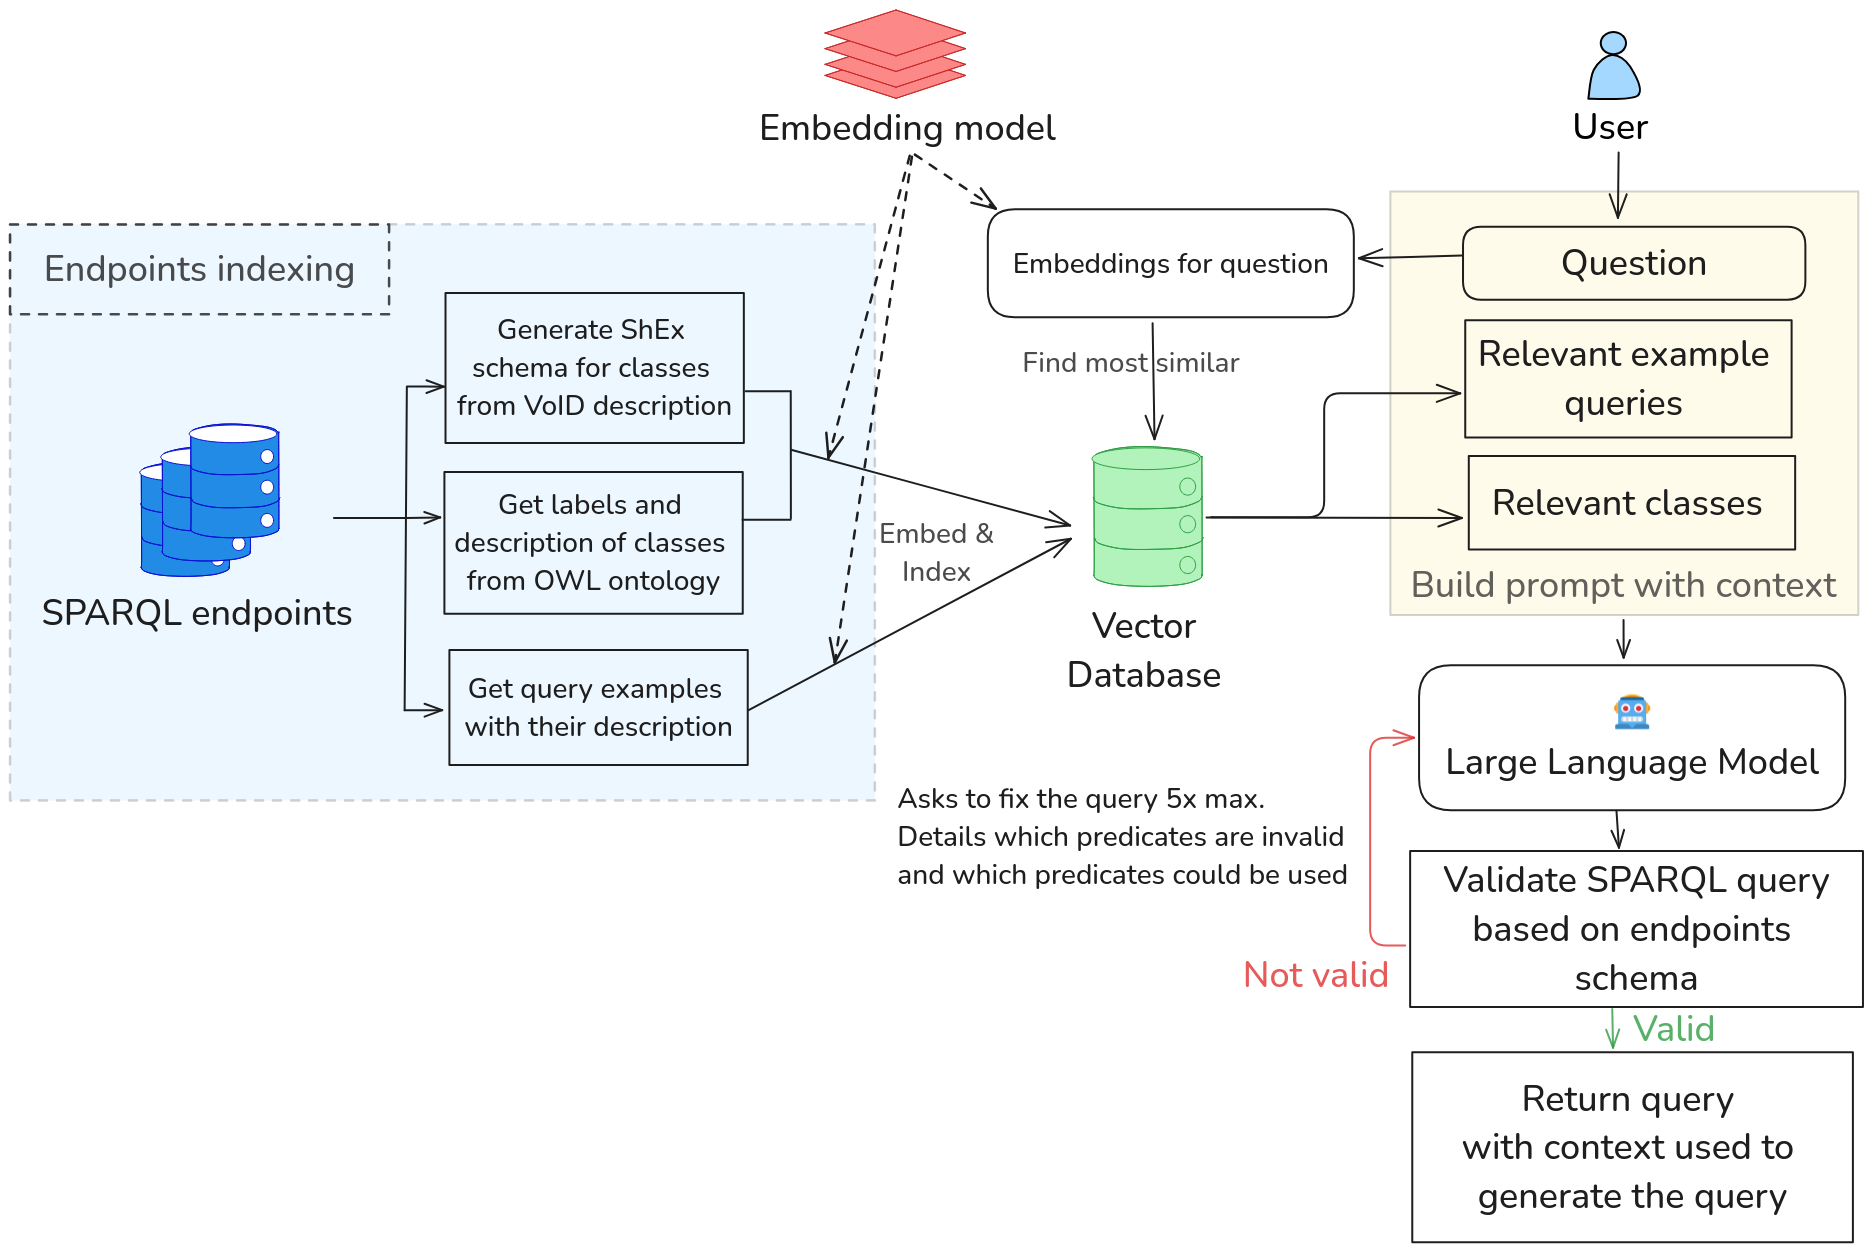
\includegraphics[width=0.95\textwidth]{expasy_architecture.png}
  \caption{LLM-based SPARQL Query Generator System Architecture.}
  \label{fig:sysarch}
\end{figure*}

% TODO: explain the process

% SysArch Figure~\ref{fig:sysarch} with system and subsections with modules:

% \begin{enumerate}
%     \item preprocessing: formatting examples (sparql-examples), extracting VoID, uploading to endpoint
%     \item endpoint indexing: extracting formatted metadata (which one)
%     \item embedding questions-queries + schema info (similarity search in Vector DB / Qdrant),
%     \item prompt tuning (elements included in prompt),
%     \item invoking LLM + validation of results using VoID to avoid schema-level hallucinations + presentation of generated query to user (showing relevant similar questions + Yasgui editor)
%     \item logging user interaction (+ mechanisms for user feedback)
% \end{enumerate} 

\subsection{Generating embeddings and indexing}

% First, we retrieve existing example question/query pairs into a vector database, such that questions asked by users can then be matched based on similarity to existing ones.
Example question/query pairs are automatically retrieved from each endpoint via a SPARQL query upon initial deployment. Embeddings are generated for each question and indexed in a vector database, allowing to match user provided inputs based on similarity search. A documented repository \cite{sparqlexamples2024} of example question/query pairs\footnote{\href{https://github.com/sib-swiss/sparql-examples}{github.com/sib-swiss/sparql-examples}} and a CLI tool\footnote{\href{https://github.com/sib-swiss/sparql-examples-utils}{github.com/sib-swiss/sparql-examples-utils}} are provided to help endpoints maintainers define and validate SPARQL query examples for their endpoints in a standardized format.


Additionally, we generate and index shapes for the classes present in each endpoint. For this, we first retrieve the VoID descriptions from each endpoint, which detail the relationships between subject classes and object classes or datatypes via specific predicates. For example, the \textit{Protein} class is linked to the \textit{Gene} class through the \textit{encodedBy} predicate. The VoID generator is available open source\footnote{\href{https://github.com/JervenBolleman/void-generator}{github.com/JervenBolleman/void-generator}} and can be used to generate statistics over any SPARQL endpoint. This information allows us to generate simple, human-readable Shape Expressions (ShEx) for each class. Each object property references a list of classes rather than another shape, making each shape self-contained and interpretable on its own.

We chose to use the ShEx schema language instead of the Web Ontology Language (OWL) for several reasons. First, endpoints may not implement all properties and classes described in the OWL ontologies they utilize, as ontologies operate under the open-world assumption. As a consequence, a more precise schema, based on the actual contents of the endpoint, must be generated for improved accuracy. Additionally, ShEx is specifically designed to express schema constraints, and its syntax is closer to the SPARQL syntax, making it more suitable for defining the structure of data in our context. In contrast, OWL requires separate classes to define properties with specified domains and ranges, resulting in a more complex and verbose representation. As a side effect, the increased verbosity would also incur higher costs due to the increase in number of tokens.

The generated shapes are well-suited for use with a LLM, as they provide information about which predicates are available for a class, and the corresponding classes or datatypes those predicates point to. For example here is the shape generated for a \textit{Disease Annotation}:

\begin{verbatim}
up:Disease_Annotation {
  a [ up:Disease_Annotation ] ;
  up:sequence [ up:Chain_Annotation up:Modified_Sequence ];
  rdfs:comment xsd:string ; up:disease IRI }
\end{verbatim}

Once the shapes have been generated, labels and descriptions are retrieved from the class OWL ontology by querying the endpoint, and then indexed in the vector database for each class. If no labels or descriptions are found, the class URI is used as the label.

%Two distinct text embeddings are generated — one using the label and the other using the description (when available) — and these are indexed in the vector database alongside the provided shape. This enables us to identify the most semantically similar classes in response to a given query and supply their schema to the LLM.
% This approach ensures coverage of classes and predicates that may not have been explicitly mentioned in the query examples.

General information about the contents of each endpoint, retrieved from the schema.org metadata available at each SPARQL endpoint homepage, are also added to the vector database. This allows to provide general information about the endpoint in case questions about it are asked by the users. 

\subsection{Prompt building}

% These elements are incorporated into the prompt alongside the user query.

When a user asks a question, embeddings are generated for the question, and the 20 most similar questions and 15 closest class labels are retrieved from the vector database. A limit is used rather than a similarity threshold to ensure the model has access to enough examples to determine whether the question can be answered based on the available endpoint data. Moreover, even if the retrieved examples have a low similarity score, they still provide hints on how to write the query, and can be useful when combined with the classes schemas. The retrieved questions and their associated queries, as well as the classes label and their associated schema, are added to the prompt alongside the user question. A concrete example of a generated prompt can be found online \footnote{\href{https://github.com/sib-swiss/sparql-llm/blob/main/notebooks/EXAMPLE_PROMPT.md}{github.com/sib-swiss/sparql-llm/blob/main/notebooks/EXAMPLE\_PROMPT.md}}.


% This allows the model to filter out irrelevant examples and class schemas, maximizing the chance of providing relevant information.
% No similarity threshold is applied, as the LLM is capable of filtering the relevant examples and class schemas. 

% When a user asks a question, we generate embeddings for this question and retrieve the most similar questions from the vector database, as well as the most similar classes labels to this question. The questions and their associated query, and the classes label and their associated schema are added to the prompt alongside the user question. An example of the generated prompt can be found online \footnote{\href{https://github.com/sib-swiss/sparql-llm/blob/main/notebooks/EXAMPLE_PROMPT.md}{github.com/sib-swiss/sparql-llm/blob/main/notebooks/EXAMPLE\_PROMPT.md}}.


% \textbf{TODO: how many}

\subsection{Validating generated queries}

To mitigate potential errors (e.g., hallucinations), we developed a method to validate federated SPARQL queries based on the VoID description of the endpoints. First, the validator parses the SPARQL query generated, which can be a federated query. Next, the validator extracts triple patterns, identifies the endpoint(s) where these will be executed, and whether the triple patterns comply with the expected schema. For each subject that has an explicit class assigned, the system will check if the stated predicates are available for this class according to the precomputed ShEx schema. The system will also try to infer the classes of other connected entities that do not have a class explicitly defined.

% For each subject that has a class, the system will check if the associated predicates are available for this class according to the schema, and it will infer the classes of other connected entities that do not have a class explicitly defined. 

% that has a certain class we check if this predicate is known to be used with this class. We also infer classes when possible if they are not provided for a subject.

%. For each endpoint involved in the generated SPARQL query, a schema is generated from the VoID description extracted from the endpoint. The validator then recursively checks whether each predicate used with a subject of a given class exists in the endpoint and furthermore is applicable to the class (according to the schema). The validator recursively examines all objects connected to this subject. In the case where an object's class is not explicitly defined, it also attempts to infer the type based on the endpoint schema.

The validator produces a list of human-readable errors describing which predicates are incorrect, the associated subject or class, and a list of valid predicates based on the schema. The errors and  corrections are then provided back to the LLM to help correct the wrong query, for example: "\textit{Subject ?disease with type up:Disease in endpoint https://sparql.uniprot.org/sparql does not support the predicate rdfs:label. It can have the following predicates: skos:altLabel, rdfs:comment, up:mnemonic, skos:prefLabel, rdfs:seeAlso}".

% \subsection{Logs and feedback}

% All user questions are stored in a log file. Additionally, the chat interface includes a simple user feedback mechanism through like/dislike buttons.

% All user questions are stored in a log file, from which they can be analysed to better understand users needs. Additionally, the chat interface includes a simple user feedback mechanism through like/dislike buttons. When one of these buttons is clicked, the entire conversation is stored in a log file in JSONL format on the server. We provide a notebook to display all conversations from the logs in a human-readable way to help maintainers analyze feedbacks.

% - for example, to prioritise the analysis of results that were disliked, in order to correct possible errors. 

% One way to achieve this is to identify extensions to the catalog of existing examples to include golden standard queries for questions that were incorrectly translated into SPARQL queries by the system.

\subsection{Context transparency and feedback}

The "\textit{See relevant references}" button in the chat interface allows users to browse the retrieved queries and classes provided as context to the LLM, along with their similarity scores. This feature enables users to investigate references and understand the reasons behind any incorrect generated query.

% There is also a "\textit{Run and edit the query}" that enables the user to automatically open the SPARQL query generated in a web editor for SPARQL that is using the same endpoint metadata used by this system to help users with contextualized classes and predicates autocomplete\footnote{\href{https://sib-swiss.github.io/sparql-editor/}{sib-swiss.github.io/sparql-editor}}.

All user questions are stored in a log file. Additionally, the chat interface includes a simple user feedback mechanism through like/dislike buttons. When one of these buttons is clicked, the entire conversation is stored in a file on the server. A notebook is provided to display all logged conversations in a human-readable way to help maintainers analyze feedbacks.



\section{Implementation}

The different components of the system are modular, published as a python package\footnote{\href{https://pypi.org/project/sparql-llm}{pypi.org/project/sparql-llm}}, and can be reused in other systems. The main components included are: 1) A module to automatically generate a human-readable ShEx schema for each class extracted from the VoID description of an endpoint, and generate documents to load in a vector database, compatible with the LangChain framework; 2) A module to automatically retrieve query examples from an endpoint and generate documents to load in a vector database; 3) A module to automatically validate a federated SPARQL query based on each endpoint VoID description, providing human-readable error messages and suggested corrections.

% The system's modular components are published as a Python package\footnote{\href{https://pypi.org/project/sparql-llm}{pypi.org/project/sparql-llm}} and can be reused in other systems. Key components include: 1) A module to generate human-readable ShEx schemas for classes extracted from an endpoint's VoID description, creating documents for a vector database compatible with the LangChain framework; 2) A module to retrieve query examples from an endpoint and generate documents for the vector database; 3) A module to validate federated SPARQL queries based on endpoint VoID descriptions, offering human-readable error messages and suggested corrections.

% \begin{itemize}
%     \item A module to automatically generate a human-readable ShEx schema for each class extracted from the VoID description of an endpoint, and generate documents to load in a vector database, compatible with the LangChain framework,
%     \item A module to automatically retrieve query examples from an endpoint and generate documents to load in a vector database, compatible with the LangChain framework,
%     \item A module to automatically validate a federated SPARQL query based on each endpoint VoID description, providing human-readable error messages and suggested corrections.
% \end{itemize} 

The system can easily support any LLM that is served via an OpenAI-compatible API. As of today, a lot of open-source inference tools and LLM cloud providers use this standard. While we primarily rely on OpenAI models, we have also been testing the system with models such as LLaMA and Mixtral.

The fastembed\footnote{\href{https://qdrant.github.io/fastembed/}{qdrant.github.io/fastembed}} library is used with the model \textit{BAAI/bge-large-en-v1.5} to generate text embeddings, chosen for its speed and high performance on the Massive Text Embedding Benchmark  \cite{muennighoff2022mteb}\cite{excoffier2024generalist}\footnote{\href{https://huggingface.co/spaces/mteb/leaderboard}{huggingface.co/spaces/mteb/leaderboard}}. The Qdrant\footnote{\href{https://qdrant.tech/}{qdrant.tech}} vector database is used to store the embeddings and perform cosine similarity search. 


% The Qdrant\footnote{\href{https://qdrant.tech/}{qdrant.tech}} vector database is used to store embeddings and perform cosine similarity search. Embeddings are generated independently of the vector database in order to keep the flexibility in choosing the embedding model. Currently we use the fastembed library which provides implementations for many popular embedding models that rank well on the Massive Text Embedding Benchmark  \cite{muennighoff2022mteb}\footnote{\href{https://huggingface.co/spaces/mteb/leaderboard}{huggingface.co/spaces/mteb/leaderboard}}. %We chose to use a generalist embedding model as it has been shown to be more efficient than specialist models for clinical semantic search\cite{excoffier2024generalist}. We are using \textbf{JINA?}


% Most of the system is written in python as this is the most popular language for data science and machine learning. It is served as an HTTP API with OpenAPI documentation. The frontend chat website is written in vanilla HTML/JavaScript and served by the python HTTP API. 

The system is containerised to facilitate reusability and deployment via docker/podman compose.

% All user questions are stored in a log file. Additionally, the chat interface includes a simple user feedback mechanism through like/dislike buttons.

\section{Evaluation and discussion}

% A number of benchmarks for question answering over knowledge graph have been published\cite{sciqa2023}\cite{Dblp-quad}, we are considering looking into implementing them for our system, but the complexity of the queries and the schema is lower to the federated system we are currently working with, which would reduce the relevance of the benchmark, so we have currently focused on making our system modular and available to the public.

We designed a preliminary test suite of 13 questions, each paired with a reference query, ensuring none are present in the examples seen by the system. The questions require reasoning over the context and specify clear retrieval tasks. For each question, the system generates a query, which we run and compare against the expected results. To account for LLM variability, each question is tested 3 times.

We assess the system's performance across three configurations: 1) baseline LLM without RAG, 2) RAG without validation, and 3) RAG with validation and correction of the generated query. This approach allows us to evaluate the contribution of each system component in improving query generation accuracy and helps detect any regressions when modifications are introduced. Additionally, the test suite is adaptable for testing different LLMs, enabling a comparison of their effectiveness in handling the questions. The results are summarised in Table~\ref{tab:model_comparison}, price is computed from average per request.

The results indicate that larger LLMs perform significantly better overall, efficiently extrapolating from provided examples. In contrast, query validation is particularly valuable for smaller LLMs, not only improving accuracy but also ensuring the system generates queries that retrieve at least some relevant results.

% We ask the system to generate a query for each question, we then run this query and compare the results obtained to the results of the expected query. Each question is tested 3 times, to reduce the impact of the probabilistic nature of LLMs responses.

% The questions are run in 3 scenarios: bare LLM without RAG, RAG without validating the generated query, RAG with validation and correction of the generated query. This enables us to test how helpful the different components of the system are at generating the right query, and to prevent regression when bringing changes to the system. The test suite can also be run on different LLMs in order to study how efficient they are at solving the questions. The results obtained are shown in 
% Table~\ref{tab:model_comparison}.

So far, our primary focus has been on developing a production system to assist users of the SIB SPARQL endpoints in formulating effective queries. In the future, we aim to conduct a more comprehensive evaluation using standardised benchmarks\cite{Dblp-quad}\cite{sciqa2023} and benchmarking frameworks\cite{meyer2024assessingsparqlcapabilitieslarge} to assess the system's precision, usability, and overall performance across a wider range of queries.

We observed that when the system retrieves context that does not fully align with the user’s question, it typically provides an answer that, while imprecise, helps guide the user towards understanding how they might answer the question using available resources. For example, when asked, "What is the function of the esophagus?" the system may return a query that lists anatomical entities with descriptions where "esophagus" appears in the name. Though not directly answering the user’s question, this query still brings the user closer to a solution by suggesting relevant resources. If the retrieved context is insufficiently relevant, the system explicitly states that it cannot answer the question.

Evaluating query results in bioinformatics is particularly challenging, even for human experts, due to the inherent complexity of both the domain-specific questions and the knowledge graph models. These challenges often introduce interpretative flexibility when determining the accuracy or relevance of the system’s outputs. As such, we expect users—typically researchers—to apply a critical approach when assessing the answers provided by the system.

The main weakness we identified in the current system is the tendency to hallucinate entity identifiers that cannot be found in examples, as well as its reliance on inefficient string comparisons that are not well optimized in SPARQL engines. To address these issues, we plan to introduce entity indexing from the endpoints, along with few-shot prompting, to enhance entity extraction and resolution.

% Evaluating query results in bioinformatics is often challenging, even for human experts, due to the inherent complexity of both the domain-specific questions and the KGs models. These complexities can introduce a degree of interpretative flexibility when assessing the accuracy or relevance of the results. As such, we still expect users, typically researchers, to apply a critical approach when evaluating the answers provided by the system.


% Given the complexity of biomedical questions and the intricate nature of the knowledge graphs we are querying, these queries often require expert-level interpretation. Questions in bioinformatics are frequently ambiguous or hard to answer, and the system’s responses should be considered as part of a larger problem-solving process. Hence, we still expect users, typically researchers, to apply a critical approach when evaluating the answers provided by the system.

% Hence, we still expect users to critically assess the answers provided by the system, especially when the retrieved examples are less relevant to their original query.
% Hence, we still expect the users to have a critical approach when considering the answer given by the system.

% We noticed that if the retrieved context does not allow to answer the user question, the system will either give a response that is a bit imprecise, but still bring the user a bit closer to how they can answer their question using the available resources, or it will say it cannot answer the question. For example, to answer the question "What is the function of the esophagus?" the system will give the query to retrieve the list of anatomical entities with their description where esophagus appears in the name. Hence, we still expect the users to have a critical approach when considering the answer given by the system. Depending of how relevant to the question the retrieved examples are, the system will either.

% In most cases we have seen the system will try to use given examples to give a response that is a bit imprecise, but still bring the user a bit closer to how they can answer their question using the available resources. For example “What is the function of the esophagus?” will give the list of anatomical entities from Bgee with their description where esophagus appears in the name. Then, it will still be the responsibility of the user to evaluate if the answer is relevant enough, and build upon this.


% In Table 1 we report the amount of correct queries generated on the 30 passes (13 questions 3 times).

% TODO: pick up some of the questions and their generated query, and try to explain why they fail. e.g. the smaller model are missing the filter on organism when asked for "the human gene LCT", while this is properly picked up by larger models.


\begin{table}
  \captionsetup{format=plain}
  \caption{Test results for different models and RAG approaches across query results categories}
  \label{tab:model_comparison}
  \begin{tabular}{lccccccc}
    \toprule
    Model & Approach & Success & Different Result & No Result & Error & Price (\$)  & F1 \\
    \midrule
    gpt-4o & No RAG & 3 & 0 & 36 & 0 & 0.00478 & 0.08 \\
    gpt-4o & RAG w/o validation & 33 & 0 & 5 & 1 & 0.03707 & 0.85 \\
    gpt-4o & RAG w/ validation & 34 & 3 & 1 & 1 & 0.04781 & 0.91 \\
    \midrule
    gpt-4o-mini & No RAG & 0 & 0 & 9 & 30 & 0.00011 & 0.0 \\
    gpt-4o-mini & RAG w/o validation & 13 & 7 & 18 & 1 & 0.00111 & 0.37 \\
    gpt-4o-mini & RAG w/ validation & 11 & 18 & 9 & 1 & 0.0019 & 0.37 \\
    \midrule
    Mixtral 8x22B & No RAG & 0 & 0 & 16 & 23 & 0.0007 & 0.0 \\
    Mixtral 8x22B & RAG w/o validation & 6 & 11 & 20 & 2 & 0.01073 & 0.18 \\
    Mixtral 8x22B & RAG w/ validation & 10 & 14 & 10 & 5 & 0.02147 & 0.31 \\
    \midrule
    Llama3.1 8B & No RAG & 0 & 0 & 6 & 33 & 8e-05 & 0.0 \\
    Llama3.1 8B & RAG w/o validation & 0 & 0 & 15 & 24 & 0.00144 & 0.0 \\
    Llama3.1 8B & RAG w/ validation & 3 & 2 & 20 & 14 & 0.00405 & 0.08 \\
    \bottomrule
  \end{tabular}
\end{table}

% - Questions / Queries pairs: how many, num triple patterns, stats on federated queries

% - Average cost per query? (\~0.035\$) average num tokens per request? (6k input, 200 output approx.)

% - Metrics : F1? Precision? Bleu/SP-Bleu (were used for the previous publication about SPARQL generation)

% - Results

% - Discussion (what systematically fails, what can be improved)

% \subsection{Future work}

% - Improving entity URIs extraction and linking

% - Driving cost down

% - Better evaluation as mentioned above.

\section{Conclusions}

We have introduced a system for generating federated SPARQL queries leveraging LLMs over real-world KGs, in response to Natural Language questions asked by users. The system currently handles questions over bioinformatics KGs within the SIB Semantic Web of Data, but can easily be reused with other KGs of interest. The system is fully open-source and a demo can be accessed online at \href{https://chat.expasy.org}{chat.expasy.org}.

\begin{acknowledgments}
We acknowledge contributions and fruitful discussions with the SIB Semantic Web Focus Group, as well as funding provided through the Biodata Resources Team at SIB. This work was also supported by the CHIST-ERA grant CHIST-ERA-22-ORD-09 by SNF grant 20CH21\_217482 and the Swiss Open Research Data Grants (CHORD) in Open Science I, a program coordinated by swissuniversities, grant id “Swiss DBGI-KM”. UniProt is supported by the National Eye Institute (NEI), National Human Genome Research Institute (NHGRI), National Heart, Lung, and Blood Institute (NHLBI), National Institute on Aging (NIA), National Institute of Allergy and Infectious Diseases (NIAID), National Institute of Diabetes and Digestive and Kidney Diseases (NIDDK), National Institute of General Medical Sciences (NIGMS), National Institute of Mental Health (NIMH), and National Cancer Institute (NCI) of the National Institutes of Health (NIH) under grant U24HG007822. UniProt activities at the SIB are additionally supported by the Swiss Federal Government through the State Secretariat for Education, Research and Innovation SERI.
\end{acknowledgments}

%%
%% Define the bibliography file to be used
\bibliography{sample-ceur}

\appendix

\section{Online Resources}

The source code for the Expasy chat system and the reusable modules.

\begin{itemize}
\item Chat system and components source code: \href{https://github.com/sib-swiss/sparql-llm}{github.com/sib-swiss/sparql-llm},
\item
  SPARQL examples example repository: \href{https://github.com/sib-swiss/sparql-examples}{github.com/sib-swiss/sparql-examples},
\item
  CLI to validate SPARQL examples: \href{https://github.com/sib-swiss/sparql-examples-utils}{github.com/sib-swiss/sparql-examples-utils},
\item
  CLI to generate VoID descriptions: \href{https://github.com/JervenBolleman/void-generator}{github.com/JervenBolleman/void-generator},
\item
  Check an endpoint metadata: \href{https://sib-swiss.github.io/sparql-editor/check}{sib-swiss.github.io/sparql-editor/check}.
\end{itemize}


\end{document}

%%
%% End of file
